%!TEX root = first try.tex

% \chapter{Case study}

% A case study to assess the feasibility of the methods/criteria developed in previous paragraphs by using both FEM software and methods/criteria. 


\chapter{Conclusion}

%Compare the result from different calculation method. Give conclusion based on the comparison result.

\begin{appendices}

\chapter{Investigation of report series created by D181 Committee Group}


\section{Introduction}

D181 Committee Group is created by UIC, in order to investigate Lateral Forces on Railway Bridges. Some of the proposed criteria in reports created by this committee group are adopted by Eurocode Committee to created Eurocode 1991-2. The goal of this investigation is to summarize the research done by D181 report series and and give further conclusion.

The investigation will be done in following aspects:

\begin{enumerate}
    \item Investigation of DT329
    \item Investigation of RP6
    \item Conclusion of D181 report series
\end{enumerate}

\subsection{Structure of report series}

Reports involved in the series are listed below in the order of publishing time:

\begin{enumerate}
    \item RP 1: Summaries of national standards and literature survey
    \item RP 2: Submitted programs and example of application
    \item RP 3: Dynamic measurements on the steel bridge over the Brenta river on the MilanVenice line at 234 + 0.963 km
    \item RP 4: Dynamic measurements on steel bridges over the Váh river by Sala on the MarcheggSzob line at 117 748 km
    \item DT 312: Etude de l'influence de la fréquence du filtre sur les valeurs mesurées des forces verticales et latérales sur les rails
    \item RP 5: Dynamic measurements on the metal arched bridge on PKP
    \item DT 313: Analyse des déformations latérales d'un pont souple (cas du PONT de LIXHE) Ligne SNCB de TONGRESMONTZEN par J.J. REBER SBB Bau GD
    \item DT 329: Parametric study Part 1: Parametric study Initial phase (September 1994) Part 2: Parametric study Phase 2 (February 1995) Authors: L.T. James and G.A. Scott
    \item RP 6: Final Report
\end{enumerate}

In this thesis DT 329 and RP 6 are obtained and studied, but other reports in English version are not available to the researcher.

\subsection{Items of interests in report series}

\begin{enumerate}
    \item Resonance mechanisms studied. They are discussed in DT329. See Section.\ref{sec:resonance329}
    \item The proposed 1.2 Hz Criterion and its background. It is discussed in RP6. See Section.\ref{sec:1.2criterion329}
    \item  Lateral forces(Nosing force) on the bridges. See Section.\ref{sec:lateralforce329}
\end{enumerate}

\section{Investigation of DT329}
\subsection{Methodology of Parametric Research DT329}

The DT329 research was conducted in two phases. It is noted that all studies were done using VAMPIRE software. The reliability of simulation has been discussed and confirmed in previous reports. 

In the initial phase 11 sets of bridge parameters were selected for the simulation. 52 combinations of bridge parameters and train configurations were examined. The goal of the initial phase is to filter out most influencing parameters for bridge dynamics.

In the secondary phase, the influence of selected parameters were categorized into 3 cases. They include:
\begin{enumerate}
 \item the influence of multiple span bridges (viaducts)
 \item the influence of track quality
 \item the influence of stiffness/span/frequency on the resonant behaviour of the bridge
\end{enumerate}
They were studied by using the same simulation method used in initial research phase.




% For the initial phase, the dynamic lateral response to the passage of different train types were examined.

% The method of modelling bridge behaviour adopted is the Theory of Normal Modes. Each train is modelled as a series of masses interconnected by suspension components of known characteristic. Time-step integrations are then performed to simulate the passage of a train over the bridge model along a track sample, which extends beyond the bridge.

% Comparisons of measured bridge responses with VAMPIRE simulations of the bridges and trains involved were the subject of earlier studies for ERRI Committee D 181, the results being documented in reports RP 3, RP 4, and RP 5 of the Committee. Each vibration model was derived from finite element analysis of the bridge structure.

% The committee have selected eleven sets of bridge parameters to be subjected to a selection of lateral load conditions. Lateral loading is provided by three train types, each running at two speeds within their respective operational ranges, on track appropriate to the train type. The combinations selected for this phase are tabulated in Appendix 1. Since the bridge design parameters are necessarily general, finite element techniques for producing bridge vibration models are inappropriate; general transverse beam vibration theory is used instead.

% For the secondary phase, as part of ERRI(UIC) investigation of Lateral Forces on Railway Bridges, the ERRI D181 Committee have commissioned British Rail Research (BRR) to carry out a parametric study(DT329) using their VAMPIRE dynamics software. 

% The study has investigated the influence of key bridge parameters and of different train types on the lateral deflections and lateral forces exerted on the bridge. The study has been carried out in two phases.

% The first phase examined 52 combinations of bridge parameters and train configurations. This study showed that some of the input parameters had little influence on the dynamic behaviour of the bridge and that others had a significant influence. There were also some parameters which appeared to show resonant effects at particular values. The results were presented in the initial report (Reference [1], part 1 of this ERRl D 181/DT 329).

% From the results of the first phase of the study, the ERRI DI81 Committee were able to select the cases for the second part in order to concentrate on those parameters which had the largest influence on the behaviour of the bridge. The cases to be considered were divided into three categories. These investigated the influence of multiple span bridges (viaducts), the influence of track quality and the influence of stiffness/span/frequency on the resonant behaviour of the bridge.



% Focus is placed on secondary phase of study of DT329, since it consists research on resonance behaviour of the bridge.

\subsection{Modelling}\label{sec:modelling329}
A special version of VAMPIRE with bridge module implemented was used to run simulation analysis. 

For an overview of modelling setup in both research phases, see Figure \ref{fig:modelling overview}. Following paragraphs will give details of modelling.


\begin{figure}[h]
\centering
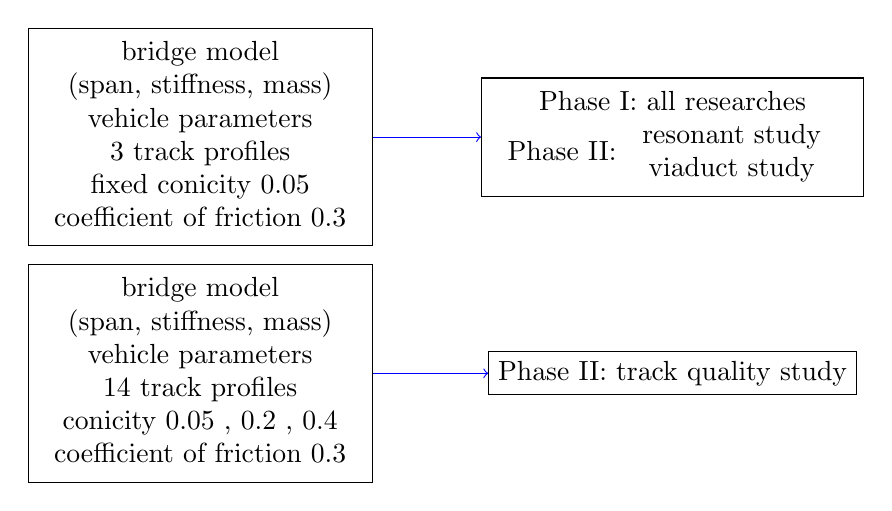
\begin{tikzpicture}

    \node[draw] (parameters) at (0,0) {
        \begin{tabular}{c}
            bridge model \\
            (span, stiffness, mass) \\
            vehicle parameters \\
            3 track profiles \\
            fixed conicity 0.05\\
            coefficient of friction 0.3 \\
        \end{tabular}
    };

    \node[draw] (phase I) at (6,0) {
        \begin{tabular}{c}
            Phase I: all researches \\
            Phase II: 
                \begin{tabular}{c}
                    resonant study\\
                    viaduct study\\
                \end{tabular} \\
        \end{tabular}
    };

    \node[draw] (phase II) at (6,-3) {Phase II: track quality study};

    \draw[->,draw=blue] (parameters) to (phase I);

    \node[draw] (parameters2) at (0,-3) {
        \begin{tabular}{c}
            bridge model \\
            (span, stiffness, mass) \\
            vehicle parameters \\
            14 track profiles \\
            conicity 0.05 , 0.2 , 0.4\\
            coefficient of friction 0.3 \\
        \end{tabular}
    };

    \draw[->,draw=blue] (parameters2) to (phase II);

\end{tikzpicture}

\caption{Overview of modelling setups for different studies conducted in DT329 }
\label{fig:modelling overview}
\end{figure}


\subsubsection{Model of bridge}
The bridge cases were modelled by assuming the bridges to behave as simply supported uniform beams. Transverse beam theory was then used to determine the frequencies and mode shapes of vibration for a given combination of span, mass per unit length and flexural rigidity. The modal information for the bridge was then used in a 'Normal Modes' analysis of the bridge.

For each case, all lateral modes of vibration up to and including 20 Hz were used. In order to prevent this artificially over-simplifying the model, if fewer than five modes were 20 Hz or less, all of the first five were used.

\subsubsection{Bridge parameters}

The spans considered were: 20 m, 33 m, 54 m, 90 m and 120 m. The flexibilities, defined as deflection of mid span over span length due to a static point load of 100 kN at mid span, are: 1/4000, 1/10000, and 1/20000. The mass per unit lengths required are: 2 tonnes/m, 6 tonnes/m, and 10 tonnes/m.

For the initial phase, see Figure \ref{fig:bridgeparametercombination} for a selection of eleven of the possible combinations examined.

\begin{figure}[h]
    \centering
    \includegraphics[width=\textwidth]{bridgeparametercombination}
    \caption{Bridge parameter combination}
    \label{fig:bridgeparametercombination}
\end{figure}

\subsubsection{Vehicle parameters}
Three train types are considered: a typical freight train, a typical standard passenger train, and a typical high speed passenger train. Appendix.\ref{app:dt329data} details the parameters used to construct each model. In general, each model consists of a locomotive and a number of identical vehicles appropriate to the train type. The total number of axles in each train is 24. Although effects on the train are only examined on the first vehicle of each type, extra vehicles are added to the train to see what cumulative effects occur to the bridge.

The freight train consists of a British Railways Class 56 locomotive and nine UIC wagons. This has a total length of 131.56 m, which assumes a nominal vehicle coupling distance of 4 m. Runs at 60 km/h and 100 km/h are required.

The standard passenger train consists of an E444 locomotive and five UIC coaches. This has a total length of 143.8 m. It is based on one of two train models used as part of the study of the FS Bridge discussed in report RP 3 of the Committee, differing only by the addition of three extra coaches. This is required to run at 160 km/h and 200 km/h.

The high speed passenger train consists of an ETR500 locomotive and five ETR500 coaches, having a total length of 145.8 m. It is based on the other FS bridge study train model mentioned above, differing from the original by an additional three ETR500 coaches. It is required to run at 300 km/h and 350 km/h.

\subsubsection{Track}

For initial study phase, the track samples used were consistent with each train type. PSD plots of each are shown in Figures \ref{fig:track1} to \ref{fig:track3}. Sample TRACKFRT.DAT was used for all analysis runs for the freight train. This is measured data from a typical BR freight line. Sample TRACKPN.DAT was used for the standard passenger train analysis runs. This is measured data from a part of the BR East Coast main line. Sample TRACKPH.DAT was used for high speed passenger train analysis runs. This is measured data from a typical DB high speed line.

Samples of 500 m were chosen so that there would be 100 m before the bridge and at least 100 m after the bridge for all combinations of span and train length. The initial 100 m is required to check vehicle behaviour on the track irregularity alone, and the portion after the train has left the bridge is required to check that the bridge vibrations decay.

For secondary study phase, the track data used to excite the mathematical models was taken from the British Rail Research library of measured track data. For the viaduct and resonance investigations, the track files used were the same as those used in the first part of the study. For the investigation of the influence of track quality, additional track data was used so as to give the widest possible range of realistic track qualities.

\subsubsection{Contact data}
For each run the same contact data was used, consisting of rails inclined at 1:20, and wheel profiles of conicity of 0.05 (based on standard British Rail 113A rails and PI wheel profiles). The coefficient of friction applied was 0.3.


\subsubsection{Data produced}

For every analysis run the following results were obtained at intervals of 0.01 seconds.

BRIDGE DATA:

Lateral displacement at mid span Lateral acceleration at mid span

\vspace*{\baselineskip}

VEHICLE LATERAL ACCELERATION DATA:

Loco body at leading pivot

Leading coach/wagon body at leading pivot/axle 

Loco leading bogie

Leading coach/wagon leading bogie/axle

\vspace*{\baselineskip}

TOTAL LATERAL FORCE DATA:

Loco leading bogie

Leading coach/wagon leading bogie/axle

\vspace*{\baselineskip}

LATERAL FORCES ON INDIVIDUAL WHEELS

Leading coach/wagon, first axle, left and right wheels 

Leading coach/wagon, second axle, left and right wheels 

Loco, first axle, left and right wheels

Loco, second axle, left and right wheels

\vspace*{\baselineskip}

In addition, for freight train runs, since the locomotive has two bogies of three axles, the forces on the individual wheels of the third axle were also produced.

Peak values for each of the outputs produced for the required ranges were obtained. For bridge outputs, peak values were taken for the period where any part of the train was on the bridge. For loco and leading coach/wagon outputs, peak values were taken whilst the vehicle in question was in contact with the bridge.

Peak values for each output were then read into a spread sheet where they could be compared more easily to check for emerging trends. The spread sheet has been partially automated to produce graphs of a single output for each train type for a single varying bridge parameter, for given values of the other bridge parameters. Figures 4 to 30(\cite{d181dt329}) show typical plots which have been produced in this manner.

\subsection{Investigation of resonance phenomenon studied in DT329}\label{sec:resonance329}

2 types of resonance were studied in DT329, including:

\begin{enumerate}
    \item Resonance caused by axle repeat pattern
    \item Resonance caused by kinematic movement
\end{enumerate}

The summary of these resonances effects are presented in following paragraphs. 

Frequency shift phenomenon is an important characteristics observed from resonance effects lists above. It is explained in Section \ref{sec:apparentshift}

\subsubsection{Resonance caused by axle repeat pattern}

Axle repeat patterns are wavelength phenomena - regardless of vehicle speed, the repeat length is constant. However, since frequency is speed divided by wavelength, the frequency of the axle repeat patterns vary with train speed. A table of axle repeat pattern lengths, and typical frequencies arising from train speed are given in Figure.\ref{tab:329axlerepeat}

By running train at different speeds shows resonance is possible between train and bridge if the axle passing frequency coincides with the first lateral bridge mode. The effect occurring in bridge lateral displacement over a limited frequency range around the resonance frequency.


However, the speed on theory which should yield resonance effect may be different from the speed that actually triggered resonance.

\subsubsection{Resonance caused by kinematic movement of trains} 
Kinematic wavelength also gives rise to frequencies which vary with speed for the same reason. For first lateral bending mode coincidence with kinematic frequency, the kinematic wavelength of each train type had to be established, by running each train at a range of typical operating speeds over a discrete lateral irregularity, and examining the frequency content of the lateral wheel motion. The resulting wavelength ranges are tabulated in Table.\ref{tab:329kinematicwavelength}. See Figure \ref{fig:workflow329kinematic} for an overview of workflow of this study.

The most likely possible resonance in the initial studies to be of this type was between the passenger train at 200 km/h (55.556 m/s) on passenger track and BR PI wheel profiles, and a span of 54 m, stiffness 1/10000, mass/length of 6 tonnes/m. This combination was examined by varying the speed between 55.556 - 64.6 m/s over the span, and by varying the stiffness of the span between 117000 and 1112000 running the train at 55.556 m/s. Another combination was examined - the ETR500 train running between 65 - 80 m/s on high speed track and BR PI wheel profiles, for a span of 38 m, stiffness 1110000, and mass/length 10 tonne/m; the span in this case was chosen to coincide with the kinematic wavelength of the coaches.

Coincidence of vehicle kinematic frequency with bridge first lateral bending mode may cause resonance to occur over a broad range of frequencies to a less pronounced effect than coincidence of axle passing frequencies. Evidence of coincidence of kinematic wavelength with length of span has been found in the lateral acceleration of bridges, but was not demonstrated in the lateral bridge displacement in the cases examined. For short kinematic wavelengths, this effect could not be seen, possibly because of lack of time for the bridge to respond.


\begin{figure}[h]
\centering
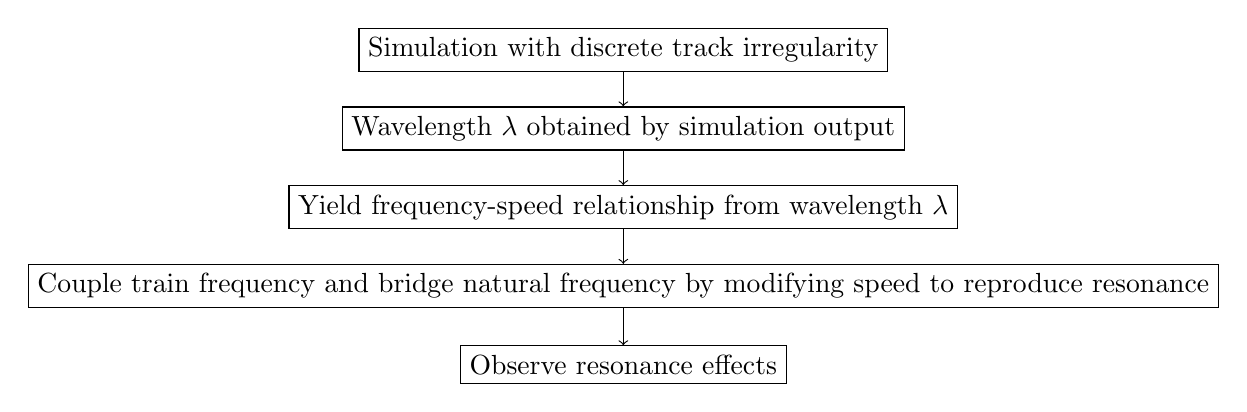
\begin{tikzpicture}
    \node[draw] (simulation1) at (0, 0) {Simulation with discrete track irregularity};

    \node[draw] (analysis) at (0, -1) {Wavelength $\lambda$ obtained by simulation output};

    \node[draw] (yielding) at (0, -2) {Yield frequency-speed relationship from wavelength $\lambda$};

    \node[draw] (matching) at (0,-3) {Couple train frequency and bridge natural frequency by modifying speed to reproduce resonance};

    \node[draw] (observe) at (0, -4) {Observe resonance effects};

    \draw[->] (simulation1) to (analysis);

    \draw[->] (analysis) to (yielding);

    \draw[->] (yielding) to (matching);

    \draw[->] (matching) to (observe);
\end{tikzpicture}
\caption{Workflow of kinematic resonance research}
\label{fig:workflow329kinematic}
\end{figure}

\subsubsection{Apparent shift in resonance frequency}\label{sec:apparentshift}
It is frequently observed in the output of both resonance effects that apparent resonance happens at some frequencies higher than frequencies calculated on theory. This is explained in following quote on \cite[Page 13, Secondary Phase]{d181dt329}. However, the explanation wasn't verified by further studies. They can only be treated as hypothesis.

\begin{quote}
Although the peak mid span displacement was expected to occur at 28.5 mis, it can be seen that for the runs with just the coaches that the peak occurs at about 32 m/s. This is confirmed to be a resonance-type effect rather than a discrete event in the time histories of the runs, a selection of which are shown in Figure C6(Original report), of which an extract of 100-285m follows as Figure C7(Original report). This speed is mid way between axle passing frequency coinciding with first bending mode of the bridge, and kinematic frequency coinciding with the first bending mode. So, the apparent shift in resonant frequency may be due to a combination of these effects (see discussion of kinematic frequency resonance results). However, an alternative explanation may be that as track forces generally increase with speed, the deflection of the span would be expected to increase. If this effect continued through a resonant band, the peak displacement would appear greater at a speed slightly above that calculated for resonance, as sketched in Figure \ref{fig:apparentshift}.
\end{quote}

\begin{figure}[h]
    \centering
    \includegraphics[width=\textwidth]{apparentshift}
    \caption{Sketch of Possible Explanation for Apparent Shift in Resonant Frequency. Extract from \cite[Appendix 2]{d181dt329}}
    \label{fig:apparentshift}
\end{figure}

In the sketch of possible explanation of apparent shift in resonant frequency(Figure \ref{fig:apparentshift}), the combined effect is the superposition of both resonance effect and speed-related effect. Speed-related effect simply increase when speed increase regardless of resonance. Speed is linear to frequency. Thus speed-related effect also simply increase when frequency increases. Resonance effect has an impact where frequency of train and bridge coincides. Speed-related effects is the cause for the frequency shift of combined peak output.

Both explanations indicate that apparent resonance frequency can hardly be predicted. Apparent frequency may even shift into domain lower than theory frequency. 


\section{Investigation of RP6}

\subsection{Debate on proposed 1.2Hz criterion}\label{sec:1.2criterion329}
Evidence of \cite{d181} is the origin of \cite[A.2.4.4.2.4(3)]{EC12} is found in \cite[p4.2: Lateral Frequencies]{d181}:

In order to avoid the phenomena of lateral resonance in vehicles, the first natural frequency of lateral vibration of the span $f_{lt}$ such that:

\begin{equation}
f_{lt} \geq 1.2Hz
\end{equation}

The statement exactly coincides with criterion A.2.4.4.2.4(3) in Eurocode 1991. It is sufficient to acknowledge D181 RP6 as the origin of criterion A.2.4.4.2.4(3) because this report is created by UIC.

The value of frequency limit, 1.2Hz is explained in \cite[p3.2: Criterion 2]{d181}:

\begin{quote}
To avoid the occurrence of resonance in the lateral motion of the vehicles due to the lateral motion of the bridge, a limit value lower than the first natural frequency $f_1t$ of the lateral vibration of the span studied should be fixed. The natural frequency for lateral movements is between 0.5 and 0.7 Hz for coaches and between 0.7 and 1 Hz for locomotives. We therefore propose a safety margin $F_{lt} \geq 1.2Hz$
\end{quote}

The original author of report RP6 Graham Scott was contacted to reveal the background of 'natural frequency for lateral movements'. Mr.Scott is still in charge of the development of software VAMPIRE and he's still active in the field. Unfortunately he was unable to remember what did 'natural frequency for lateral movements' stand for in previous quotes since it was written nearly 20 years ago. He passed me to his colleague Alan Minnis for further questions. Mr.Minnis stated following:

\begin{quote}
Looking at the values I think they would refer to typical rigid body modes of a vehicle.  These are independent of speed and a typical passenger coach with air suspension will have a lower sway frequency of around 0.6Hz which is within 0.5-0.7Hz.  Locomotives tend to have a slightly stiffer suspension hence the slightly higher frequency range.
\end{quote}

Mr.Minnis statements, combined with results yielded in supporting parametric report DT329 proves 1.2Hz criterion is aiming to avoid occurrence of resonance. But this isn't a feasible strategy in following reasons:

\begin{enumerate} 
    \item The resonance between rigid body mode of train and first lateral vibration mode of the bridge has never been discussed in all D181 report series. No research proofed this kind of resonance can be critical in real life scenario.

    \item There are lots of evidence can be found in report DT329, showing resonance can happen on a bridge with a first lateral natural frequency even higher than 1.2Hz, which is self-conflicting with 1.2Hz criterion. In fact, the resonance could happen at any frequency on theory. However, the magnitude of resonance effect ranges from less pronounced to more pronounced from case to case.  

    For example, \cite[Page 14,Phase II]{d181dt329} shows resonance occurs on 1.71Hz:
        \begin{quote}
            The first lateral bending mode of this bridge is at 1. 71 Hz. The kinematic wavelength of the passenger coaches is around 34-38 m, giving a kinematic frequency range of 1.46 - 1.63Hz.Speeds of 58.14 m/s(1.53-1.71 Hz)and 64.6m/s(1.7-1.9Hz)were also done. The mid span lateral displacement for each of the time histories are shown in Figure C12(Orignial report). The slowest speed appears to show the greatest resonance.
        \end{quote}
\end{enumerate}

\subsection{Lateral forces on railway bridges}\label{sec:lateralforce329}
It is concluded in initial phase of the study that presence of the bridge doesn't influence the track forces and track quality is a major factor in determining the lateral forces generated by a particular train on \cite[Page 7, Secondary Phase]{d181dt329}

\begin{quote}
    From the initial study [1], it was concluded that the track quality on a bridge is a major factor in determining the lateral forces generated by a particular train. The D181 Committee therefore asked BRR to determine the peak track forces generated over a wide range of track qualities.

    The length of a bridge is small compared to the overall length of a railway track and so track quality on a single bridge may not be representative of that on other bridges on the same route. However the initial study concluded that, in general, the lateral track forces are not influenced by the presence of the bridge.
\end{quote}

The resonance effects mentioned in the previous sections were only observed in deflection and acceleration domain due to the reason that the presence of the bridge doesn't influence the track forces. 


Influence on the total lateral force as a result of hunting of single vehicle bodies were examined. Three parameters were involved in this parametric research. They were vehicle speed, track irregularities deviation and wheel conicity.

Vehicle speed plays a key role. When speed is 60 km/h for freight trains, in the response output, there is very limited influence by increasing both track deviation and conicity. Different conicity tends to yield same force output. Same as track deviation. See Figure B1.

When speed increases, output of different conicity on same track deviation is more scattered. Similarly, increased deviation yields yields greater output. They are two basic trends observed in all output data.

However, it is uncertain which conicity will yield greater output compared to other 2 conicity setups. Surprisingly, in some cases, best maintained wheel profile (effective conicity 0.05) generates greater output than poorly maintained wheels (effective conicity 0.4). See Figure B2. The most obvious case of this kind is freight train running at 100 km/h on track with 5.7mm (approximate) deviation.

Different from conicity, the influence of increasing track deviation is simply predictable. Research report DT329 provided approximate linear function for relationship between lateral force and track deviation. These linear functions can be extracted from plots B1-B30 of DT329.

Since peak force output of 120 km/h freight train and 200 km/h passenger train are close(2\% difference), it is reasonable to conclude that passenger train tends to yield smaller result than freight train at same speed. This is probably due to passenger trains have more sophisticated suspension system designed to suppress lateral motion of the vehicle. Unfortunately, only one speed of 200km/h configuration was available in DT329. But since freight train yields greater output, it is conservative for designer to adopt force output of freight trains for speeds of 60km/h, 100km/h, 120km/h.

It is worthy to point out a suspicious mistake of DT329 in Table.\ref{tab:peaklateralforce}. Report claimed that output data were filtered by statistical analysis. The peak lateral track force was determined from a statistical analysis of lateral track forces as $M \pm 3\sigma$ where $M$ is the mean lateral force value over the segment and $\sigma$ is the standard deviation over the segment. It does not give a true maximum lateral force but on which is greater than 99.5\% of all force values. It is obvious in Table.\ref{tab:peaklateralforce} that output data of 160kN for freight train wagon was not filtered by statistical analysis. It is the greatest value among all raw output data of freight train running at 100 km/h. See Figure B7. This data of 160kN also illustrates that 
peak forces will be influenced by discrete features in the track geometry which may not be reflected thoroughly in the standard deviation. This thesis report suggest substitute 160kN with 80kN(value by approximate observation). See Table.[note1]\ref{tab:peaklateralforce}

\begin{table}[h!]
    \centering
    \caption{Peak Lateral Track Force Over All Track Qualities. Extracted From \cite[Tab. B1]{d181dt329}}
    \begin{tabular}{cccc}
        \hline
        Peak lateral force(kN) & Locomotive Total & Coach/Wagon & Total \\ 
        \hline
        Freight 60 km/h & 50 & 60 & 110\\
        Freight 100 km/h & 90 & 160(\textbf{\textit{80}})$^1$ & 250(\textbf{\textit{170}})$^1$\\
        Freight 120 km/h & 75 & 110 & 185 \\
        Passenger 200 km/h & 140 & 50 & 190 \\
        High Speed 350 km/h & 125 & 125 & 250 \\
        Passenger 200 km/h(worn wheels) & 190 & 80 & 270 \\
        High Speed 350 km/h(worn wheels) & 330 & 225 & 555 \\
        \hline
    \end{tabular}
    \begin{flushleft}
    Note1: Force value 160kN for wagon of freight train running at 100 km/h is not representative. But it is not filtered by statistical analysis. It is advised to substitute 160kN with 80kN. 80kN is obtained by approximate observation of \cite[Figure B7]{d181dt329}. As a result, total force is reduced from 250kN to 170kN.
    \end{flushleft}
    \label{tab:peaklateralforce}
\end{table}

Speed and track quality are two most sensitive parameters. Control of track quality is more advisable compared to control of wheel conicity due to the reason that influence of track quality deviation is simply approximate linear to force output, whereas influence of wheel conicity has an unpredictable characteristic.

Figure.\ref{fig:peaklateralforceregression} is created to plot total peak force illustrated in Table.\ref{tab:peaklateralforce}. 5 sets of data available were used to create the plot. 3 of them are data of freight train running at 60km/h, 100km/h and 120km/h. The other 2 sets of data are passenger train running at 200km/h and high speed train running at 350km/h respectively. Data produced with worn wheels profiles are neglected because they are not representative for normally maintained railway vehicles. Adjacent points were connected by solid lines. Different colour stands for different train types. Red lines and dots stand for freight trains. Blue stands for passenger trains and black stands for high speed trains. 

It is indicated that freight trains tends to have the biggest lateral force on track compared to other two kind of trains. And high speed train has lowest lateral force on track. This can be explained by freight trains possessing the most stiff suspension systems, while high speed trains possessing complicated suspension system to suppress lateral motion.

It can also be concluded that the relationship between lateral force and speed is not linear. As a general phenomenon observed, force increment decreases as speed increases. Regressions were made to better illustrate the trend of lateral force increment. Please note these regressions are only sufficient within the speed range plotted.

The first regression made was on freight train because it has the most sets of data. The form of function should satisfy:

\begin{enumerate}  
    \item 0kN lateral force when speed is 0km/h
    \item Simply increasing in value but generally decreasing in increment
\end{enumerate}

Finally function form $F=a*v^b$ is selected because its satisfying characteristics. R language was used to perform regression process. The regression result is also in good likelihood with original data. Achieved convergence tolerance was 2.868e-06. The result is presented in Formula.\ref{for:regressionfreight}. See Appendix.\ref{sec:Rregression} for code.

\begin{equation}
\label{for:regressionfreight}
F_{lf} = 5.2064\cdot v^{0.7495}
\end{equation}

Since 1 set of data is available for passenger train, Formula.\ref{for:regressionfreight} is scaled by a constant factor to create regression for passenger trains. Please note that this regression can not be verified because lack of data. However, since freight train has a greater lateral force then passenger train, it is conservative to adopt lateral force of freight train when calculating consequences related to passenger trains. It is still reasonable to adopt this regression since passenger trains are just simply less stiff than freight trains. 

Unfortunately, conducting such transient simulations is extremely time and resource consuming. It is impossible for this thesis to carry out more simulations to verify the sufficiency of following scaled regression. More data on passenger train and high speed train is recommended to be produced by future researches.

The scale factor $k_{pf}$ is obtained by comparing force value yielded by Formula.\ref{for:regressionfreight} at 200km/h and original passenger train force(190kN) data at 200km/h.

$$k_{pf} = \frac{190}{a_{lf}\cdot 200^{b_{lf}}}$$
$$a_{lp} = a_{lf}\cdot k_{pf}$$
merge above two equations, yield
$$a_{lp} = \frac{190}{200^{b_{lf}}} = \frac{190}{200^{0.7495}} \approx 3.58$$

and 

$$F_{lp} = a_{lp}\cdot v^{0.7495}$$

thus

\begin{equation}\label{for:regressionpassenger}
F_{lp} = 3.58\cdot v^{0.7495}
\end{equation}

Lateral force for high speed train were obtained in same manner. The scale factor $k_{hf}$ is obtained by comparing force value yielded by Formula.\ref{for:regressionfreight} at 350km/h and original high speed train force(250kN) data at 350km/h.

$$k_{hf} = \frac{250}{a_{lf}\cdot 350^{b_{lf}}}$$
$$a_{lh} = a_{lf}\cdot k_{hf}$$
merge above two equations, yield
$$a_{lh} = \frac{250}{350^{b_{lf}}} = \frac{250}{350^{0.7495}} \approx 3.10$$

and 

$$F_{lh} = a_{lh}\cdot v^{0.7495}$$
thus

\begin{equation}\label{for:regressionhighspeed}
F_{lh} = 3.10\cdot v^{0.7495}
\end{equation}


\begin{figure}[h]
    \centering
    \begin{tikzpicture}
    \begin{axis}[
    % title = {Peak lateral track forces over all track qualities(worn profile scenario neglected)},
    xlabel={$v(km/s)$},
    ylabel={$F(kN)$},
    ymin = 0, xmin = 0, xmax = 350,
    grid = both,
    ytick = {50,100,...,250},
    xtick = {60,100,120,200,350},
    legend style={
    at={(0,0)},
    anchor=north west,at={(axis description cs:0,-0.1)}}] 
    ]
    \addplot[name path = C,mark=*] coordinates {(200,190) (350,250)};
    \addplot[blue,name path = B,mark=*] coordinates {(120,185) (200,190)};
    \addplot[red,name path = A,mark=*] coordinates {(0,0) (60,110) (100,170) (120,185)};
    \addplot[red,name path = D, domain = 0:120, dashed]{5.2064*x^0.7498};
    \addplot[blue,name path = E, domain = 0:200, dashed]{3.58*x^0.7498};
    \addplot[name path = F, domain = 0:350, dashed]{3.1*x^0.7498};
    \legend{high speed train, passenger train, freight train, approximate freight train ,approximate passenger train, approximate high speed train},
    \end{axis}
\end{tikzpicture}
\caption{Total peak lateral track forces over all track qualities(worn profile scenario neglected)}
\label{fig:peaklateralforceregression}
\end{figure}
Formula\ref{for:regressionfreight},\ref{for:regressionpassenger} and \ref{for:regressionhighspeed} can be used as load forces for different design scenario. However, these loads are normally higher than the load defined in EN1991-2\cite[6.5.2 Nosing force]{EC12}. EN 1991-2 states that the characteristic value of the nosing force shall be taken as $Q_sk = 100 kN$. 

It is worthy to note that although in RP6\cite[Proposed criteria]{d181} several load model with loading magnitude ranging from 70 kN to 270 kN were originally proposed, EN1991-2 uses a single characteristic value of 100 kN for all design scenarios. 

Since no document has explained this modification, this is probably due to the consideration of lower track irregularity deviation during the creation of EN1991-2.

As explained in previous chapter, peak force is generally linear to track standard deviation. Most of the peak lateral force described in DT329 was obtained on track with 7mm standard deviation, while EN13848-5\cite{13848} allows much lower track standard deviation defined in Table \ref{tab:lateraldeviation}. This means peak lateral force on tracks(if maintained according to Eurocode regulations) in European Union is also much smaller than peak force obtained in DT329. 

EN1991-2 states the usage of nosing force 
 



\section{Conclusion of D181 report series}
The report series managed to create load models for lateral dynamics railway effects. It is worthy to note that the lateral force on the track wasn't influenced by the presence of the bridge. The major influencing parameter for lateral force is track quality and conicity of the wheel profile. 

The resonance phenomenon was successfully reproduced and observed, though its only visible in deflection and acceleration domain. A basic characteristic of resonance, regardless of the type of resonance, is that apparent resonance frequency will shift from resonance frequency calculated on theory. The shift is unpredictable in the sense of both direction and magnitude. The effect related to speed start to creep in when speed is higher, making the effect of resonance less pronounced in higher speed(Figure \ref{fig:apparentshift}). 

Please note that every bridge will always have resonance with running train because axle repeat pattern and kinematic movement are both wavelength phenomenon, which means there is always a speed of train yielding a vibration frequency coincides with the first lateral natural frequency of bridge. However, the effect of resonance happening on long-span bridge is usually unpronounced since the speed of the train is low as 2.5m/s to 14m/s when resonance occurs.  

Some of the conclusion and proposed criteria in RP6 were adopted in Eurocode 1991-2. One of them is 1.2Hz criterion. It was adopted without amending. The other one is lateral force models. They were adopted in a different name as 'nosing force' in \cite[A6.5.2]{EC12}. 

The 1.2Hz criterion was under debate and proofed unreliable in fulfilling its original intention, avoiding occurrence of resonance. There is no research in D181 report series supporting this criterion, nor there exists literature behind the natural frequency of vehicles. This criterion ignored the fact of future bridge designs with long span would certainly have a natural frequency lower than 1.2 Hz. It is advised that Eurocode review this criterion and revise it.


\chapter{Plots and diagrams used in D181 DT 329}\label{app:dt329data}

\begin{figure}[h]
    \centering
    \includegraphics[width=\textwidth]{vp11}
    \caption{BR CLASS 56 LOCOMOTIVE. Extract from \cite[Appendix 2]{d181dt329}}
\end{figure}

\begin{figure}[h]
    \centering
    \includegraphics[width=\textwidth]{vp12}
    \caption{BR CLASS 56 LOCOMOTIVE. Extract from \cite[Appendix 2]{d181dt329}}
\end{figure}

\begin{figure}[h]
    \centering
    \includegraphics[width=\textwidth]{vp21}
    \caption{UIC FREIGHT WAGON (LADEN). Extract from \cite[Appendix 2]{d181dt329}}
\end{figure}

\begin{figure}[h]
    \centering
    \includegraphics[width=\textwidth]{vp22}
    \caption{UIC FREIGHT WAGON (LADEN). Extract from \cite[Appendix 2]{d181dt329}}
\end{figure}

\begin{figure}[h]
    \centering
    \includegraphics[width=\textwidth]{vp31}
    \caption{FS ETR500 LOCOMOTIVE. Extract from \cite[Appendix 2]{d181dt329}}
\end{figure}

\begin{figure}[h]
    \centering
    \includegraphics[width=\textwidth]{vp32}
    \caption{FS ETR500 LOCOMOTIVE. Extract from \cite[Appendix 2]{d181dt329}}
\end{figure}

\begin{figure}[h]
    \centering
    \includegraphics[width=\textwidth]{vp41}
    \caption{FS ETR500 COACH. Extract from \cite[Appendix 2]{d181dt329}}
\end{figure}

\begin{figure}[h]
    \centering
    \includegraphics[width=\textwidth]{vp42}
    \caption{FS ETR500 COACH. Extract from \cite[Appendix 2]{d181dt329}}
\end{figure}

\begin{figure}[h]
    \centering
    \includegraphics[width=\textwidth]{vp51}
    \caption{FS E444 LOCOMOTIVE. Extract from \cite[Appendix 2]{d181dt329}}
\end{figure}

\begin{figure}[h]
    \centering
    \includegraphics[width=\textwidth]{vp52}
    \caption{FS E444 LOCOMOTIVE. Extract from \cite[Appendix 2]{d181dt329}}
\end{figure}

\begin{figure}[h]
    \centering
    \includegraphics[width=\textwidth]{vp61}
    \caption{UIC COACH. Extract from \cite[Appendix 2]{d181dt329}}
\end{figure}

\begin{figure}[h]
    \centering
    \includegraphics[width=\textwidth]{vp62}
    \caption{UIC COACH. Extract from \cite[Appendix 2]{d181dt329}}
\end{figure}

\begin{figure}[h]    \centering
    \includegraphics[width=\textwidth]{track1}
    \caption{Horizontal track irregularities for freight trains. Extract from \cite[Figure 2.1]{d181}}
    \label{fig:track1}
\end{figure}

\begin{figure}[h]
    \centering
    \includegraphics[width=\textwidth]{track2}
    \caption{Horizontal track irregularities for standard passenger trains. Extract from \cite[Figure 2.1]{d181}}
\end{figure}

\begin{figure}[h]
    \centering
    \includegraphics[width=\textwidth]{track3}
    \caption{Horizontal track irregularities for high speed passenger train. Extract from \cite[Figure 2.1]{d181}}
    \label{fig:track3}
\end{figure}

\begin{table}[h]
    \centering
    \begin{tabular}{c|c|c|c}
    \hline
    \multirow{2}{*}{Freight train: Principle axle repeat patterns} & dist & \multicolumn{2}{c}{Speed} \\
    & m & 60 km/h & 100 km/h \\
    \hline
    wagon n axle 2 - wagon n+1 axle 1 & 4.00 & 4.17 & 6.94 \\
    wagon wheelbase & 9.00 & 1.85 & 3.09 \\
    wagon n axle m - wagon n+1 axle m & 13.0 & 1.28 & 2.14 \\
    wagon n axle m - wagon n+2 axle m & 26.0 & 0.64 & 1.07 \\
    \hline
    \multirow{2}{*}{Passenger train: Principle axle repeat patterns} & dist & \multicolumn{2}{c}{Speed} \\
    & m & 160 km/h & 200 km/h \\
    \hline
    coach n axle 1 - 2, and coach n axle 3 - 4 & 2.56 & 17.36 & 21.70 \\
    coach n axle m - coach n+1 axle m & 26.4 & 1.68 & 2.10 \\
    coach n axle m - coach n+2 axle m & 52.8 & 0.84 & 1.05 \\
    \hline
    \multirow{2}{*}{ETR 500 train: Principle axle repeat patterns} & dist & \multicolumn{2}{c}{Speed} \\
    & m & 300 km/h & 350 km/h \\
    \hline
    coach n axle 1 - 2 and coach n axle 3 - 4 & 3.0 & 27.78 & 32.41 \\
    coach n axle m - coach n+1 axle m & 26.1 & 3.19 & 3.72 \\
    coach n axle m - coach n+2 axle m & 52.2 & 1.60 & 1.86 \\
    coach n axle m - coach n+3 axle m & 69.3 & 1.20 & 1.40 \\
    \hline
    \end{tabular}
    \caption{Axle repeat patterns and typical frequencies. Extracted from \cite[Appendix C]{d181dt329}}
    \label{tab:329axlerepeat}
\end{table}

\begin{table}[h]
    \centering
    \begin{tabular}{c|c|c|c}
    \hline
    Kinematic wavelength, m & Freight train & Passenger train & ETR500 train \\
    \hline
    Locomotive & 39 - 45 & 32 - 38 & 39 - 45 \\
    Coach/wagon & 24 - 39 & 34 - 38 & 36 - 40 \\
    \hline
    \end{tabular}
    \caption{Kinematic wavelength ranges per vehicle, with BR P1 profiles. Extracted from \cite[Appendix C]{d181dt329}}
    \label{tab:329kinematicwavelength}
\end{table}

\chapter{Speeds which do not require dynamic compatibility checks} \label{app:speedsafe}

\begin{figure}[h]
    \centering
    \includegraphics[width=0.7\textwidth]{speedsafe.pdf}
    \caption{Speed limit (in km/h) in relationship Line Category/Locomotive Class and vehicle type. Extract from \cite[Appendix F]{EC15528}}
\end{figure}


\begin{figure}[h]
    \centering
    \includegraphics[width=\textwidth]{lateralloadcasesample}
    \caption{LATERAL WHEEL AND AXLE FORCES FOR BRIDGES. Extract from \cite[Fig 3.1]{d181}}
    \label{fig:lateralloadcasesample}
\end{figure}

\chapter{MU-Groups and MU-Classes}\label{app:mu}

\section{Definition}
Multiple units can be grouped according to type of traffic service(high speed - long distance, intercity - regional and commuter/suburban) or to the kind of running gear (conventional bogies, articulated bogies and single axles).


In some cases due to potential excessive dynamic load effects in bridge line category checks are not sufficient to demonstrate compatibility. To minimise the need for undertaking a dynamic check of individual trains, several typical and wide spread MU-designs have been grouped in MU-classes. For these groups of vehicles, load models covering the specified design parameter ranges have been developed to allow the efficient dynamic analysis of bridges. For practical reasons, the number of MU classes was limited and for trains outside the range of parameters covered, the process of checking an individual train existing at the time of publication of this standard as state of the art shall be used.

Each MU-class is defined by:

\begin{enumerate}[-]
\item ranges of train parameters covered and;
\item a corresponding load model for carrying out dynamic checks on bridges.
\end{enumerate}

Each MU-Group comprises of serveral MU-Classes. Table

\begin{table}[h]
    \centering
    \begin{tabular}{c|c}
        \hline
        MU-Group & MU-Class\\
        \hline
        \multirow{2}{*}{conventional bogie(CB)} & $CB_1$ \\
        & $CB_2$ \\
        \hline
        \multirow{4}{*}{articulated bogie(AB)} & $AB_1$ \\
        & $AB_2$ \\
        & $AB_3$ \\
        & $AB_4$ \\
        \hline
        \multirow{2}{*}{single axle(SA)} & $SA_1$ \\
        & $SA_2$ \\
        \hline
    \end{tabular}
    \caption{Relationship MU-groups - MU-classes}
    \label{tab:MU}
\end{table} 

\begin{figure}[h]
\centering
\includegraphics[width=0.8\textwidth]{trainparameters.pdf}
\caption{Train parameters related to MU-Groups. Extracted from \cite[Annex C]{EC15528}}
\label{fig:trainparameters}
\end{figure}

\begin{table}[h]
    \centering
    \begin{tabular}{c|c|c}
    \hline
    Name & Parameter & Unit \\
    $2a^*$ & Bogie spacing between pivot centres within a vehicle & m \\
    $2a^+$ & Axle spacing in bogie & m \\
    $u1+u2$ & Bogie spacing between pivot centres of adjacent vehicles & m \\
    $u3$ & Overhang of end coaches & m \\
    L\_Coa & Coach length & m \\
    No\_Coa & Number of coaches within an unit & - \\
    No\_Units & Number of units within a train & - \\
    \hline
    \end{tabular}
    \caption{Explanation of train parameters. Extracted from \cite[Annex C]{EC15528}}
    \label{tab:explanationtrainparameters}
\end{table}

\subsection{Train parameters of MU-Class CB\_1}

\begin{table}[h]
    \centering
    \begin{tabular}{c|c}
    \hline
    max No\_Units & 2 \\
    max No\_Coa & 8 \\
    L\_Coa & $23.8m \leq L\_Coa \leq 25.3m $ \\
    $2a^*$ & $16.8m \leq 2a^* \leq 18.0m $ \\
    $2a^+$ & $2m \leq 2a^+ \leq 3m $ \\
    $(u1+u2)$ & $7.0m \leq (u1+u2) \leq 7.6m $ \\
    $u3$ & $4m \leq u3 \leq 6m $ \\
    \hline
    \end{tabular}
    \caption{Train parameters for conformity with MU-Class CB\_1}
    \label{tab:CB1}
\end{table}

\subsection{Train parameters of MU-Class CB\_2}

\begin{table}[h]
    \centering
    \begin{tabular}{c|c}
    \hline
    max No\_Units & 2 \\
    max No\_Coa & 7 \\
    L\_Coa & $ 25.3 m \leq L\_Coa \leq 27.5 m $ \\
    $2a^*$ & $ 18.0 m \leq 2a^* \leq 19.5 m $ \\
    $2a^+$ & $ 2 m \leq 2a^+ \leq 3m $ \\
    $(u1+u2)$ & $7.2m \leq (u1+u2) \leq 8.0 m $ \\
    $u3$ & $4m \leq u3 \leq 6m $ \\
    \hline
    \end{tabular}
    \caption{Train parameters for conformity with MU-Class CB\_2}
    \label{tab:CB2}
\end{table}


\subsection{Train parameters of MU-Class AB\_1}

\begin{table}[h]
    \centering
    \begin{tabular}{c|c}
    \hline
    max No\_Units & 4 \\
    max No\_Coa & 5 \\
    $2a^*$ & $ 14.9 m \leq 2a^* \leq 16.0 m $ \\
    $2a^+$ & $ 2 m \leq 2a^+ \leq 3m $ \\
    $u3$ & $3m \leq u3 \leq 5.5m $ \\
    \hline
    \end{tabular}
    \caption{Train parameters for conformity with MU-Class AB\_1}
    \label{tab:AB1}
\end{table}

\subsection{Train parameters of MU-Class AB\_2}

\begin{table}[h]
    \centering
    \begin{tabular}{c|c}
    \hline
    max No\_Units & 4 \\
    max No\_Coa & 5 \\
    $2a^*$ & $ 18.8 m \leq 2a^* \leq 19.5 m $ \\
    $2a^+$ & $ 2 m \leq 2a^+ \leq 3m $ \\
    $u3$ & $3m \leq u3 \leq 5.5m $ \\
    \hline
    \end{tabular}
    \caption{Train parameters for conformity with MU-Class AB\_2}
    \label{tab:AB2}
\end{table}

\subsection{Train parameters of MU-Class AB\_3}

\begin{table}[h]
    \centering
    \begin{tabular}{c|c}
    \hline
    max No\_Units & 2 \\
    max No\_Coa & 11 \\
    $2a^*$ & $ 17.0 m \leq 2a^* \leq 17.5 m $ \\
    $2a^+$ & $ 2 m \leq 2a^+ \leq 3m $ \\
    $u3$ & $4.5m \leq u3 \leq 5.7m $ \\
    \hline
    \end{tabular}
    \caption{Train parameters for conformity with MU-Class AB\_3}
    \label{tab:AB3}
\end{table}

\subsection{Train parameters of MU-Class AB\_4}

\begin{table}[h]
    \centering
    \begin{tabular}{c|c}
    \hline
    max No\_Units & 2 \\
    max No\_Coa & 10 \\
    $2a^*$ & $ 18.7 m \leq 2a^* \leq 19.2 m $ \\
    $2a^+$ & $ 2 m \leq 2a^+ \leq 3m $ \\
    $u3$ & $4.3m \leq u3 \leq 5.3m $ \\
    \hline
    \end{tabular}
    \caption{Train parameters for conformity with MU-Class AB\_4}
    \label{tab:AB4}
\end{table}

\subsection{Train parameters of MU-Class SA\_1}

\begin{table}[h]
    \centering
    \begin{tabular}{c|c}
    \hline
    max No\_Units & 3 \\
    max No\_Coa & 10 \\
    $2a^*$ & $ 9.2 m \leq 2a^* \leq 9.8 m $ \\
    $u3$ & $4.25m \leq u3 \leq 6.25m $ \\
    \hline
    \end{tabular}
    \caption{Train parameters for conformity with MU-Class SA\_1}
    \label{tab:SA1}
\end{table}

\subsection{Train parameters of MU-Class SA\_2}

\begin{table}[h]
    \centering
    \begin{tabular}{c|c}
    \hline
    max No\_Units & 2 \\
    max No\_Coa & 14 \\
    $2a^*$ & $ 12.8 m \leq 2a^* \leq 13.5 m $ \\
    $u3$ & $4.25m \leq u3 \leq 6.25m $ \\
    \hline
    \end{tabular}
    \caption{Train parameters for conformity with MU-Class SA\_1}
    \label{tab:SA1}
\end{table}

\chapter{Regression commands for R console}\label{sec:Rregression}

\begin{lstlisting}[keywordstyle=\bfseries\color{blue},language=R]
> F <- c(0,110,170,185)
> v <- c(0,60,100,120)
> f <- function(a,b,v) {a*v^b}
> dat <- data.frame(v,F)
> dat
    v   F
1   0   0
2  60 110
3 100 170
4 120 185

> fm <- nls(F ~ f(a,b,v), data = dat, start = c(a=1, b=1))
> fm
Nonlinear regression model
  model: F ~ f(a, b, v)
   data: dat
     a      b 
5.2064 0.7498 
 residual sum-of-squares: 47.84

Number of iterations to convergence: 6 
Achieved convergence tolerance: 2.868e-06
\end{lstlisting}

\chapter{Train vehicles}

\section{Locomotives}
\subsection{4-axle locomotives}
Generally, the relevant parameters for categorisation of 4-axle locomotives are axle load P (18 t to 22,5 t) and the bogie axle spacing (2,2 m to 3,4 m).

Typically the mass per unit length is less than 6,4 t/m and the distance from the end axle to the end of the nearest coupling plane is greater than 1,9 m

\subsection{6-axle locomotives}

Generally, the relevant parameters for categorisation of 6-axle locomotives are:

\begin{enumerate}[-]
\item the maximum axle load P (18 t to 22 t) in combination with;
\item the distance between axles within a bogie (1,80 m to 2,25 m).
\end{enumerate}

Typically, the mass per unit length (p) is less than 6,4 t/m and the distance from end axle to the end of the nearest coupling plane (a) is greater than 2,1 m.

\section{Trains in Netherlands}

Passenger trains now in service include following models:

\begin{enumerate}
    \item The DD-AR (Dubbeldeksaggloregiomaterieel) \\  EMUs were delivered as DDM-2/3 resembling the bilevel rail cars series DDM-1 from 1985 and operates in fixed formations of 3 or 4 coaches. 4 car trains use a class 1700 locomotive for traction, 3 car trains use an mDDM motorcar, which resembles a DD-AR driving trailer but has electric motors and a single passenger deck on top; the level of this deck is higher than that of a regular single deck rail car, but lower than the upper deck of the other coaches. Three types of coaches are available: Bv (second class), ABv (first and second class) and Bvk (second class driving trailer). The DDM-2/3 series are being modernised from 2010–2013 and after modernisation the series was renamed as NID (Nieuwe Intercity Dubbeldekker).
    \item The VIRM (Verlengd Interregiomaterieel) \\ also called Regiorunner was partially rebuilt from trainsets DD-IRM (Dubbeldeks Interregiomaterieel). DD-IRM was delivered in 3- and 4-car trainsets. 3-car trainsets got one extra coach, 4-car trainsets got two extra coaches. Also, new 4- and 6-car trainsets were built. Thus, a train consists of one or more combinations of 4 or 6 double deck coaches; each combination (multiple unit) has electric motors. More than three hundred coaches are currently operative in the Netherlands.
    \item The Koploper (ICM) (Intercitymaterieel) \\ is a 3- or 4-car multiple unit that when coupled with another one, allows passengers to walk through (the name Koploper being a play on words – literally "head walker", but in actual use meaning "front runner"). The Dutch Railway Company decided to close the heads permanently on 31 October 2005 because the mechanism broke down too often. A scheduled modernisation of around 7 million euro will see the ICM fleet updated. The renovated ICM trains provide 13\% more seats (reducing the leg room to uncomfortable small for the long haul journeys they serve in 2nd class, which is further aggravated by a waste bin that is placed on the backsides of the seats in front), have a new interior, a bathroom accessible by wheelchairs, airconditioning as well as upgrades to the engine and connection systems. The head doors are removed. Also, these (renovated) trains are the first trains in the NS fleet equipped with OBIS. OBIS provides a (free) WiFi-connection on board, along with in-train journey information provided through screens and (automated) vocal announcements through the trains speakers. This journey information provides the actual status, and thus is always up-to-date to the actual situation this trip, and the stations is passes.
    \item The Sprinter (SGM, Stads Gewestelijk Materieel) \\ is a two or three car electric, used on small distances. They are named Sprinter because they're able to accelerate and brake quite fast, making them very suitable for 'stoptrein' services. They were also specifically designed for urban environments where they run commuter services. As a result, they are most commonly found in the Randstad area. The initial idea was that the Sprinter would provide somewhat of a subway/metro service but this plan failed as the cities of Amsterdam and Rotterdam continued to construct their own rapid transit systems. Nevertheless, in the densely populated Randstad, the Sprinters remain popular. Two car versions were revised and renamed to Citypendel. All Sprinters are now refurbished into the new white/yellow/dark blue livery.
\end{enumerate}
\end{appendices}